\documentclass[preview]{standalone}

\usepackage{amsmath}
\usepackage{amssymb}
\usepackage{tikz}
\usepackage{stellar}
\usepackage{definitions}

\begin{document}

\id{jordan-canonical-form-exercises}
\genpage

\section{Exercises}

\begin{snippetexercise}{jordan-form-eight-dimensional-matrix-exercise}{Jordan form of an eight-dimensional matrix}
    Determine the Jordan canonical form over \(\complexnumbers\) of
    \[
        A=
        \begin{pmatrix}
            2&0&0&0&0&0&0&0\\
            0&2&0&0&0&0&0&0\\
            0&3&1&0&1&0&0&0\\
            4&0&0&2&0&1&0&1\\
            0&0&0&0&1&2&0&0\\
            0&0&0&0&0&1&0&1\\
            0&0&0&0&0&0&2&0\\
            0&0&0&0&0&0&1&2
        \end{pmatrix}.
    \]
    Its eigenvalues are \(1\) and \(2\).
\end{snippetexercise}

\begin{snippetsolution}{jordan-form-eight-dimensional-matrix-solution}{Jordan form of an eight-dimensional matrix}
    The characteristic polynomial is
    \[
        \chi_A(T)=(T-1)^3(T-2)^5.
    \]
    For the eigenvalue \(1\),
    \[
        \mrank(A-I_8)=7,\qquad
        \mrank((A-I_8)^2)=6,\qquad
        \mrank((A-I_8)^3)=5.
    \]
    The corresponding nullities are \(1,2,3\), so there is one block
    of size at least \(1\), one of size at least \(2\), and one of size
    at least \(3\). The \(1\)-primary part is therefore \(J_3(1)\).

    For the eigenvalue \(2\),
    \[
        \mrank(A-2I_8)=5,\qquad
        \mrank((A-2I_8)^2)=4,\qquad
        \mrank((A-2I_8)^3)=3.
    \]
    The nullities are \(3,4,5\). Hence there are three blocks, exactly
    one of which has size at least \(2\), and exactly one of which has
    size at least \(3\). Their sizes are \(3,1,1\). Thus
    \[
        J(A)=J_3(1)\oplus J_3(2)\oplus J_1(2)\oplus J_1(2).
    \]
\end{snippetsolution}

\begin{snippetexercise}{jordan-form-similar-matrices-exercise}{Distinguishing similar matrices}
    Determine which of the matrices
    \[
        A=
        \begin{pmatrix}
            2&0&0&0\\
            0&2&0&0\\
            2&0&2&1\\
            0&0&0&2
        \end{pmatrix},
        \qquad
        B=
        \begin{pmatrix}
            1&1&0&0\\
            -1&3&0&0\\
            -1&1&1&1\\
            -1&1&-1&3
        \end{pmatrix},
    \]
    \[
        C=
        \begin{pmatrix}
            2&1&1&-1\\
            0&1&1&-1\\
            0&-1&3&-1\\
            0&0&0&2
        \end{pmatrix}
    \]
    are similar over \(\complexnumbers\).
\end{snippetexercise}

\begin{snippetsolution}{jordan-form-similar-matrices-solution}{Distinguishing similar matrices}
    All three matrices have characteristic polynomial \((X-2)^4\).
    Moreover,
    \[
        \mrank(A-2I_4)=1,
        \qquad
        \mrank(B-2I_4)=2,
        \qquad
        \mrank(C-2I_4)=2,
    \]
    with
    \[
        (B-2I_4)^2=0,
        \qquad
        \mrank((C-2I_4)^2)=1,
        \qquad
        (C-2I_4)^3=0.
    \]
    It follows that
    \[
        J(A)=J_2(2)\oplus J_1(2)\oplus J_1(2),
        \qquad
        J(B)=J_2(2)\oplus J_2(2),
    \]
    \[
        J(C)=J_3(2)\oplus J_1(2).
    \]
    Therefore the three matrices are pairwise non-similar:
    \[
        A\nsim B,
        \qquad
        A\nsim C,
        \qquad
        B\nsim C.
    \]
    Notice that
    \[
        \mu_A=\mu_B=(X-2)^2,
        \qquad
        \mu_C=(X-2)^3.
    \]
    Thus the minimal polynomial distinguishes \(C\), but not \(A\)
    from \(B\); the complete block decomposition is needed for the
    latter pair.

    The corresponding column diagrams are
    \[
        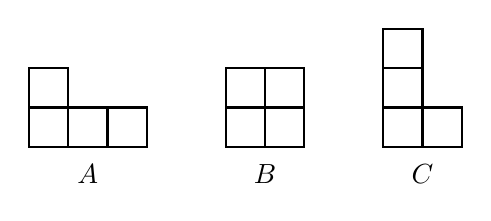
\begin{tikzpicture}[scale=0.5]
            \foreach \x/\h in {0/2,1/1,2/1} {
                \foreach \y in {1,...,\h} {
                    \draw[thick] (\x,\y-1) rectangle (\x+1,\y);
                }
            }
            \node at (1.5,-0.7) {\(A\)};

            \begin{scope}[xshift=5cm]
                \foreach \x/\h in {0/2,1/2} {
                    \foreach \y in {1,...,\h} {
                        \draw[thick] (\x,\y-1) rectangle (\x+1,\y);
                    }
                }
                \node at (1,-0.7) {\(B\)};
            \end{scope}

            \begin{scope}[xshift=9cm]
                \foreach \x/\h in {0/3,1/1} {
                    \foreach \y in {1,...,\h} {
                        \draw[thick] (\x,\y-1) rectangle (\x+1,\y);
                    }
                }
                \node at (1,-0.7) {\(C\)};
            \end{scope}
        \end{tikzpicture}
    \]
\end{snippetsolution}

\begin{snippetexercise}{jordan-form-three-parameters-exercise}{Jordan form with three parameters}
    Let \(\alpha,\beta,\gamma\in\complexnumbers\), and consider
    \[
        A=
        \begin{pmatrix}
            1&0&0&\gamma\\
            0&1&0&0\\
            0&\alpha&4&-3\\
            0&\beta&3&-2
        \end{pmatrix}.
    \]
    Determine the Jordan canonical form of \(A\) in terms of
    \(\alpha,\beta,\gamma\).
\end{snippetexercise}

\begin{snippetsolution}{jordan-form-three-parameters-solution}{Jordan form with three parameters}
    The characteristic polynomial is
    \[
        \chi_A(X)
        =(X-1)^2
        \det\begin{pmatrix}X-4&3\\-3&X+2\end{pmatrix}
        =(X-1)^4.
    \]
    Put \(N=A-I_4\). Then
    \[
        N=
        \begin{pmatrix}
            0&0&0&\gamma\\
            0&0&0&0\\
            0&\alpha&3&-3\\
            0&\beta&3&-3
        \end{pmatrix},
    \]
    \[
        N^2=
        \begin{pmatrix}
            0&\gamma\beta&3\gamma&-3\gamma\\
            0&0&0&0\\
            0&3(\alpha-\beta)&0&0\\
            0&3(\alpha-\beta)&0&0
        \end{pmatrix},
        \qquad
        N^3=
        \begin{pmatrix}
            0&3\gamma(\alpha-\beta)&0&0\\
            0&0&0&0\\
            0&0&0&0\\
            0&0&0&0
        \end{pmatrix},
    \]
    and \(N^4=0\). The ranks are consequently
    \[
        \begin{array}{c|ccc}
            &\mrank N&\mrank N^2&\mrank N^3\\
            \hline
            \gamma=0,\ \alpha=\beta&1&0&0\\
            \gamma=0,\ \alpha\neq\beta&2&1&0\\
            \gamma\neq0,\ \alpha=\beta&2&1&0\\
            \gamma\neq0,\ \alpha\neq\beta&3&2&1
        \end{array}
    \]
    and therefore
    \[
        J(A)=
        \begin{cases}
            J_2(1)\oplus J_1(1)\oplus J_1(1),
                &\gamma=0,\ \alpha=\beta,\\
            J_3(1)\oplus J_1(1),
                &\gamma=0,\ \alpha\neq\beta,\\
            J_3(1)\oplus J_1(1),
                &\gamma\neq0,\ \alpha=\beta,\\
            J_4(1),
                &\gamma\neq0,\ \alpha\neq\beta.
        \end{cases}
    \]
\end{snippetsolution}

\end{document}
